\documentclass{article}
\usepackage[utf8]{inputenc}
\usepackage{graphicx}
\setlength{\parindent}{0pt}
\setlength{\parskip}{1em}

\title{FOAR705 - Proof of Concept Elaboration I}
\author{Jan Jugueta - 44828020}
\date{29th of August 2019}

\begin{document}

\maketitle

\section*{Research Topic}

Alot has changed in the past week in relation to my Masters of Research thesis. During that time, I have had several meetings with different academic lecturers and mentors. I believe this is the first time that I had a clear idea of what Masters of Research topic will be, along with what specific sources I will use.

My research will focus on how the East German state used their state-owned media in the lead up to the 1974 FIFA World Cup. This particular World Cup is of significance to both West and East Germany, because the World Cup finals were to be held in West Germany, whilst it would the first time that East Germany would compete in the finals. To top it all off, East Germany were drawn to play West Germany in the group stage.

This research will involve obtaining newspaper articles about the World Cup from \textit{Neues Deutschland}, the pre-eminent East German newspaper. The search will limit itself to the year leading up to the World Cup till the end of 1974. A semiotic analysis of the articles content will also be performed. With these two distinct steps, I then propose two different Proof of Concepts. 

I have not entirely decided to throw away my old Proof of Concept proposed in Scoping II, however, I do feel that this proposal will be more beneficial to my workflow.

\section*{Objective}

Build on Scoping II exercise with an Elaboration for a potential process that can be used in my research project.

\newpage
\section*{Proof of Concept I - Finding and downloading newspaper articles from \textit{Neues Deutschland}}

\begin{figure}
    \centering
    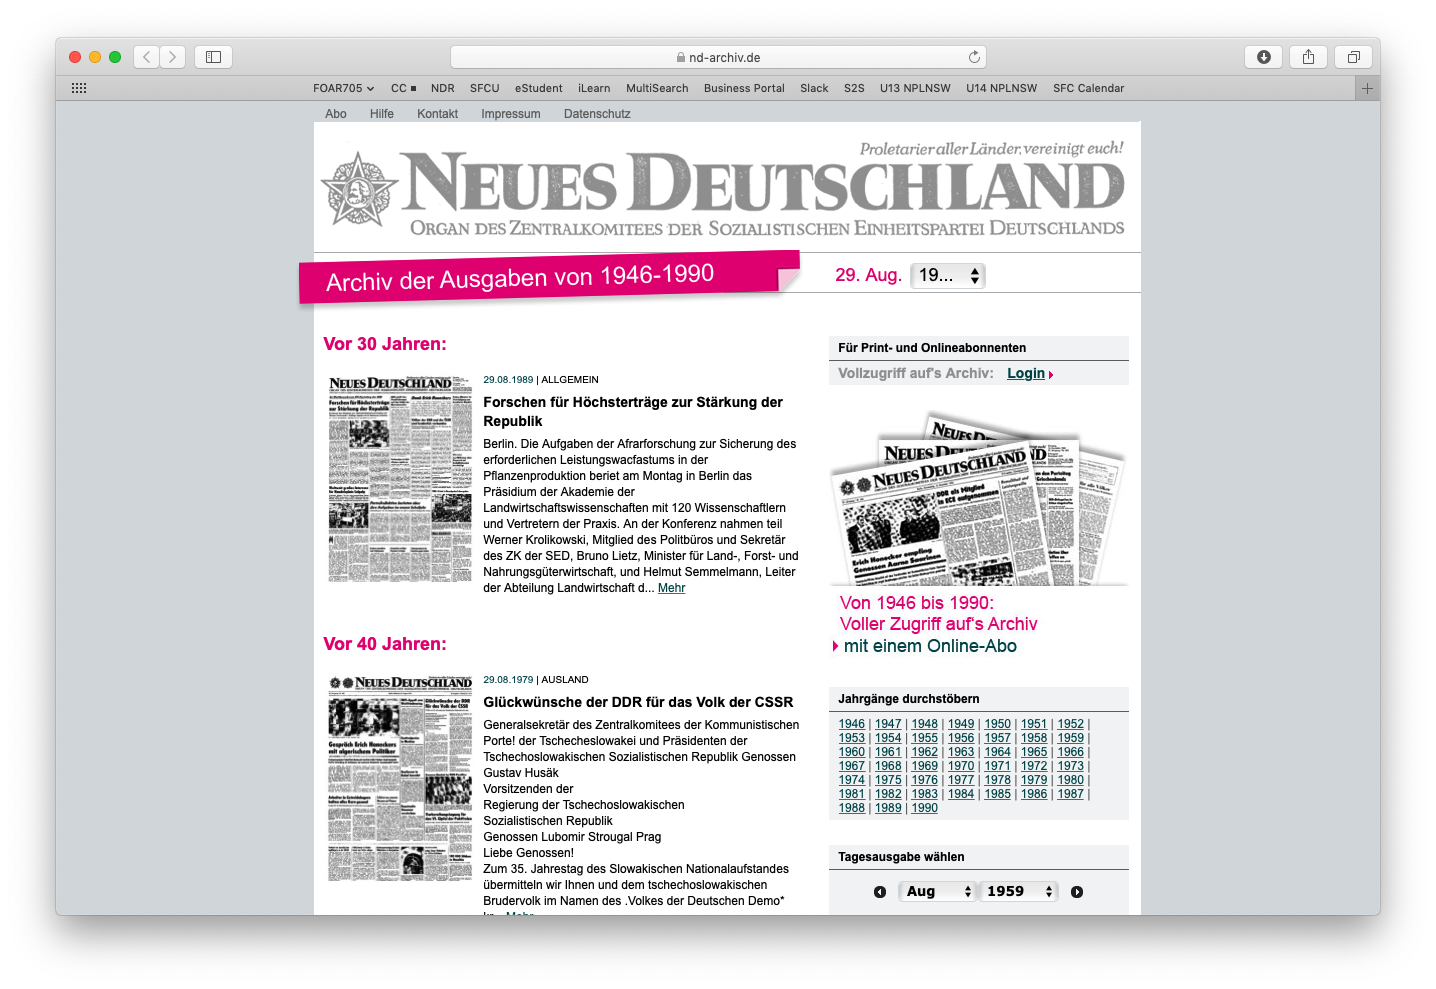
\includegraphics[width=\textwidth]{nd.png}
    \caption{\textit{Neues Deutschland website}}
    \label{fig:my_label}
\end{figure}


\textit{Neues Deutschland} was an organ for the Central Committee of the Socialist United Party in East Germany. They were in effect, the direct mouth piece of the ruling party. The website nd-archiv.de contains all newspaper articles published by the magazine from 1946 to 1990. I am currently in the process of organising an archive log in with my supervisor.

Below will outline a step-by-step process that will find all articles with the term \textit{Weltmeisterschaft} (World Cup) between January 1st 1973 and December 31st 1974.

\begin{enumerate}
    \item Enter 'weltmeisterschaft' in the \textit{Suchausdruck}.
    \item Change the date range from 1st January 1973 to 31st of December 1974 in the \textit{In welchem Zeitraum} field.
    \item Leave all other fields to default setting.
    \item Click \textit{Suchen}.
\end{enumerate}

\begin{figure}
    \centering
    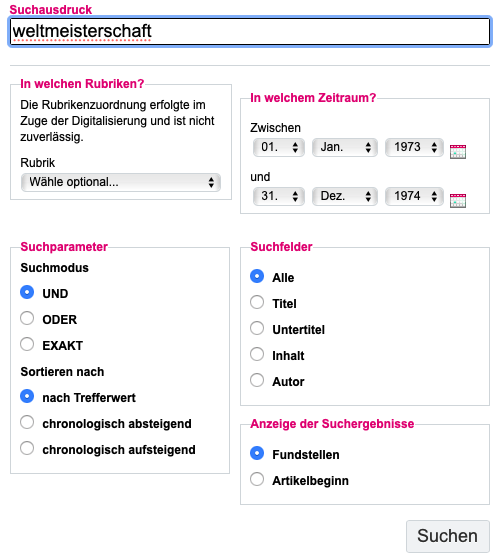
\includegraphics[width=\textwidth]{nd_search.png}
    \caption{\textit{Search Window}}
    \label{fig:my_label}
\end{figure}

From this search result, we can see that it has returned more than 100 articles that match the criteria we have entered.

\begin{figure}
    \centering
    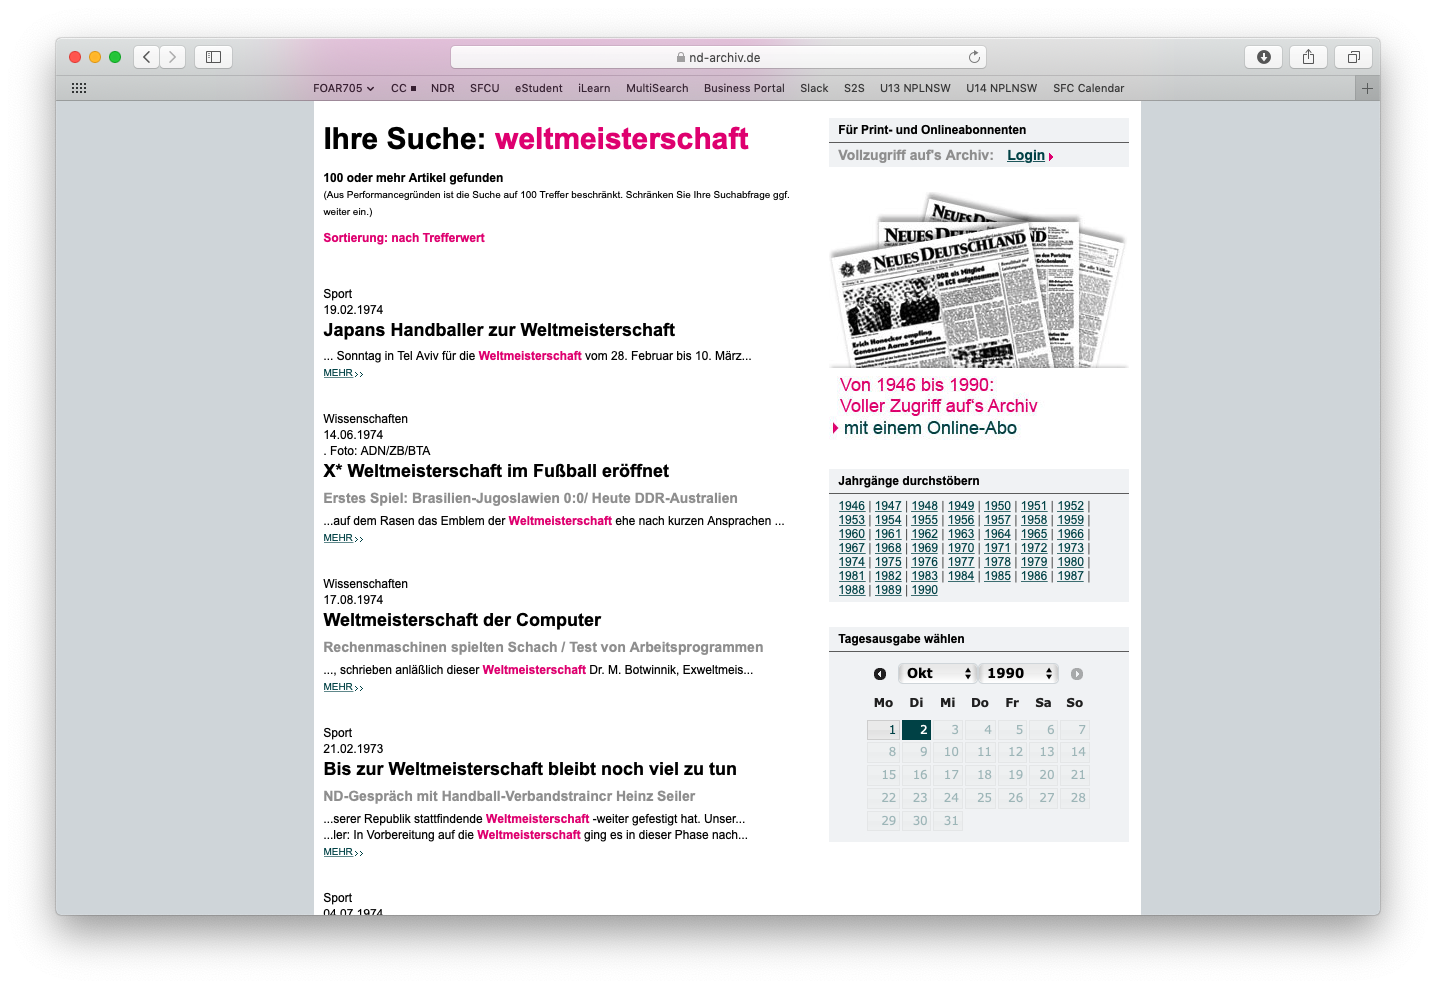
\includegraphics[width=\textwidth]{nd_searchresult.png}
    \caption{Search Result}
    \label{fig:my_label}
\end{figure}

Here comes the part of the process that becomes rather repetitive. The process is as follows.

\begin{enumerate}
    \item Click on the first article returned in the result.
    \item Copy the text from the article into a .txt (or .rtf) file.
    \item Save and name the .txt (or .rtf) into a directory stored on my machine.
    \item Go back to the website and continue this process with the next search result.
    \item Continue this process until all articles are copied.
\end{enumerate}

Once this process is completed, I should have all articles that reference 'Weltmeisterschaft' on my computer.

\section*{Proof of Concept I - Textual analysis of the corpus using Voyant Tools}

For testing this concept, I have created .rtf files in a directory on my machine that contain German-text articles about football.

\begin{figure}[h!]
    \centering
    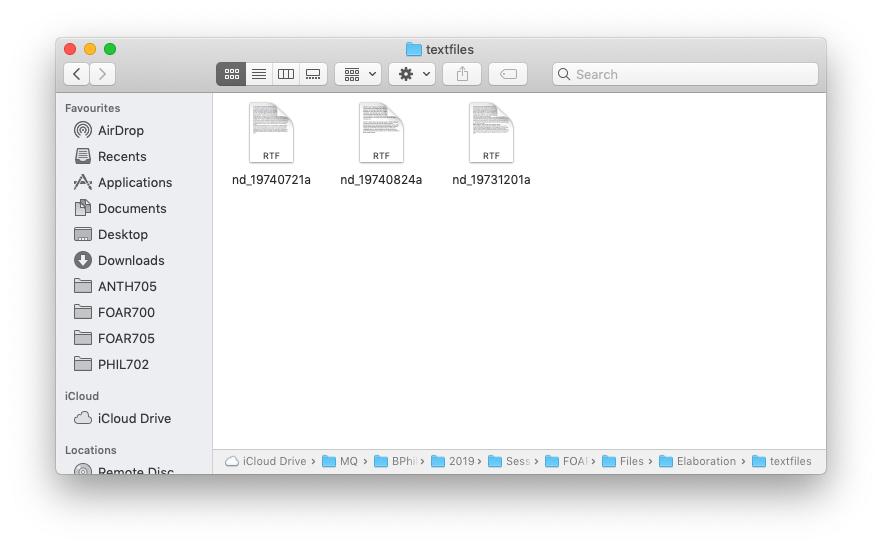
\includegraphics[width=\textwidth]{textfiles.png}
    \caption{Directory with .rtf files on my computer}
    \label{fig:my_label}
\end{figure}

Using the 'upload' function on the Voyant Tools website, I can select all my corpus files and have them analyzed by Voyant Tools.

\begin{figure}[h!]
    \centering
    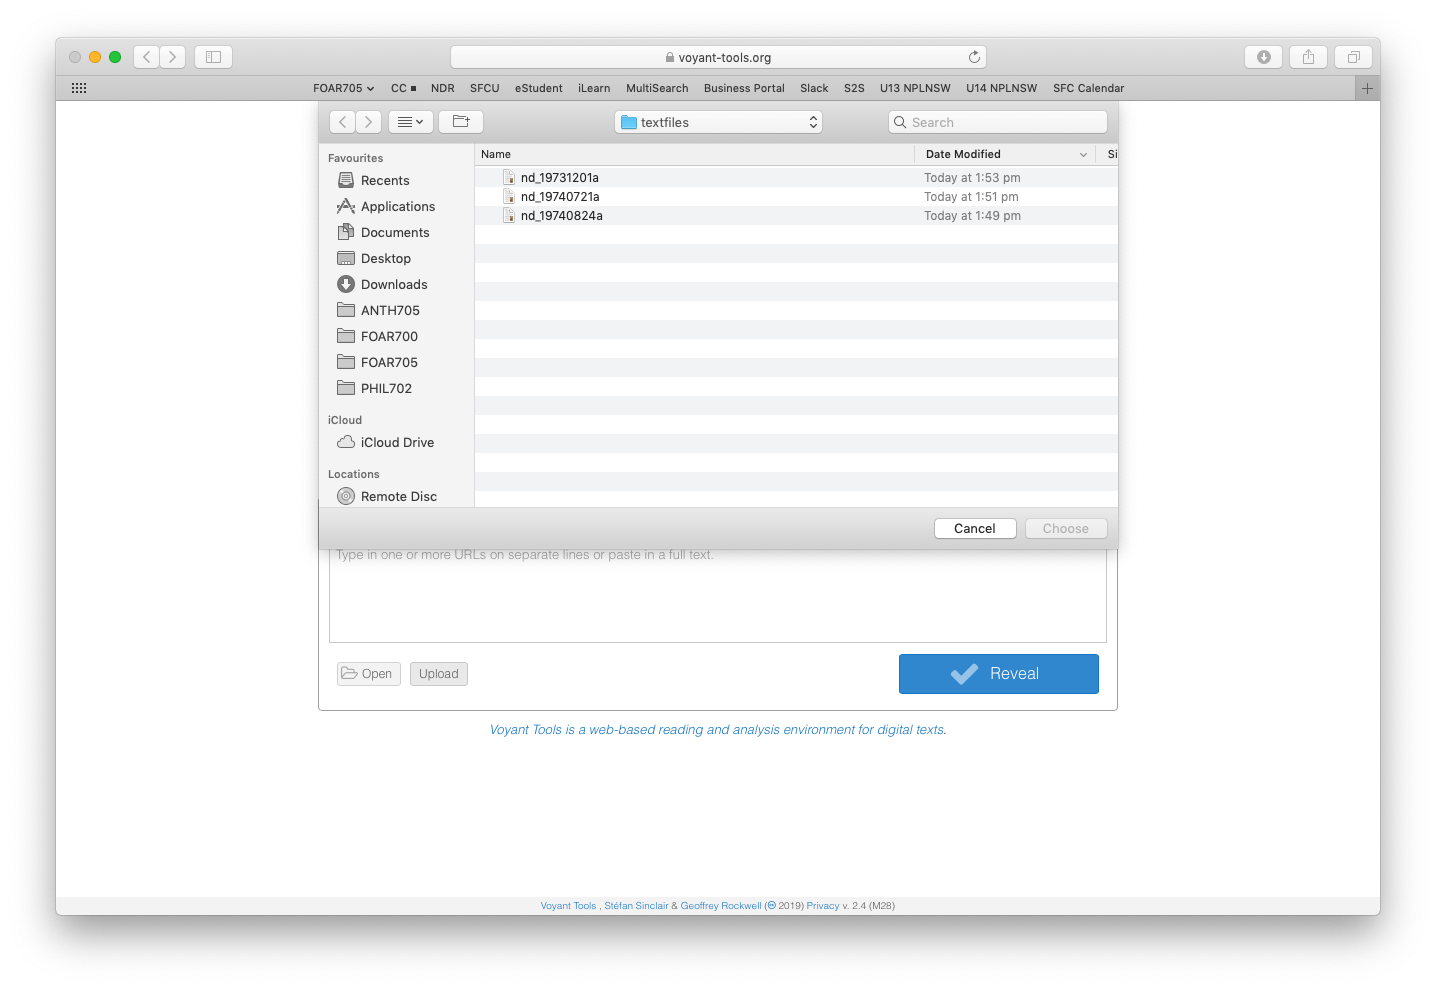
\includegraphics[scale=0.15]{voyantupload.png}
    \caption{Voyant Tools upload window}
    \label{fig:my_label}
\end{figure}

Once uploaded, I can use Voyant to analyze the corpus a number of ways. I have yet to decide which specific methodology I will employ, however, it is more than likely that Voyant will be beneficial whichever way I choose to go.

\begin{figure}[h!]
    \centering
    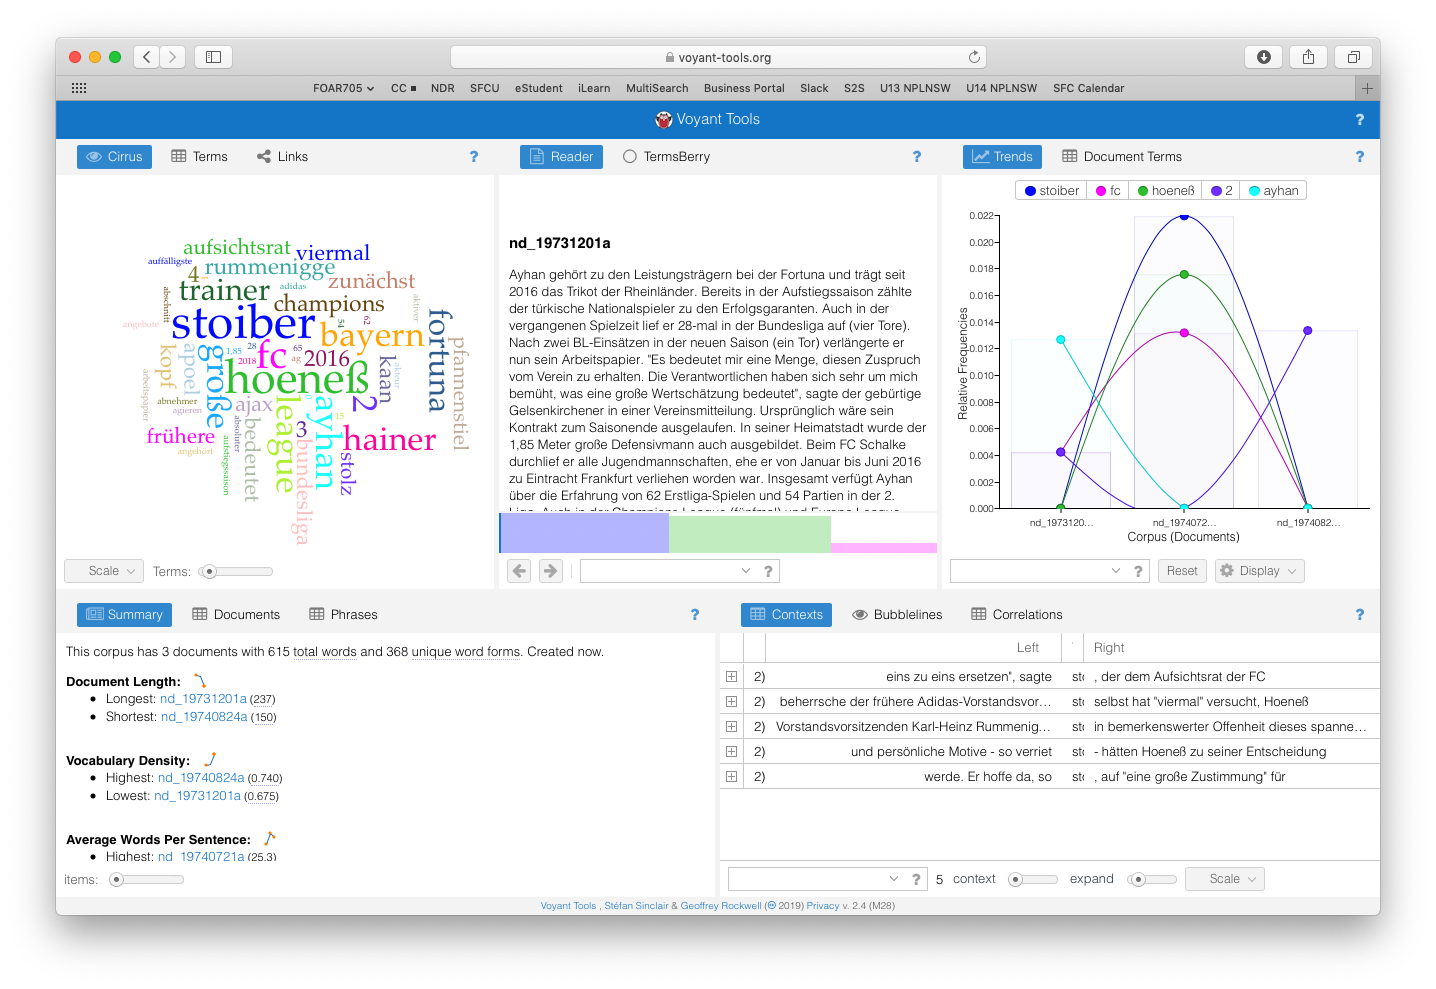
\includegraphics[width=\textwidth]{voyantresult.png}
    \caption{Voyant Tool's analysis of the corpus.}
    \label{fig:my_label}
\end{figure}

\section*{Errors}

Whilst testing the step-by-step process I have outlined, I experienced no errors. I do expect, that if I were to automate this process using Terminal or R (I'm not sure what is involved with that yet), that errors will occur.

\section*{Result}

Both Proof of Concepts seem viable and achievable within the constrains I have. I am also happy that I have figured out a potential process that will make the collation and analysis of data flow quicker and smoother.

\end{document}
